\documentclass[10pt,a4paper]{article}

\usepackage[T1]{fontenc}
\usepackage[utf8]{inputenc}
\usepackage[slovene]{babel}
\usepackage{lmodern}
\usepackage{microtype}
\usepackage{geometry}
\usepackage{amsmath,amssymb}
\usepackage{booktabs,tabularx,array}
\usepackage[table]{xcolor}
\usepackage{enumitem}
\usepackage{fancyhdr}
\usepackage[most]{tcolorbox}
\usepackage{tikz}
\usetikzlibrary{trees}

\geometry{margin=1.7cm}
\setlength{\parindent}{0pt}
\setlength{\parskip}{3pt}
\setlist[enumerate]{nosep,leftmargin=*}
\setlist[itemize]{nosep,leftmargin=*}
\renewcommand{\arraystretch}{1.2}
\definecolor{navy}{HTML}{174A7E}
\definecolor{pale}{HTML}{EEF4F8}
\definecolor{borderblue}{HTML}{9DB8CE}
\pagestyle{fancy}
\fancyhf{}
\lhead{\small Pregled snovi}
\rhead{\small Kombinatorika}
\cfoot{\thepage}
\renewcommand{\headrulewidth}{0.4pt}

\newcommand{\formula}[1]{%
    \par\smallskip\noindent
    \colorbox{pale}{\parbox{\dimexpr\linewidth-2\fboxsep\relax}{\centering\(\displaystyle #1\)}}%
    \par\smallskip}
\newcommand{\zgled}{\par\smallskip\noindent\textcolor{navy}{\textbf{Zgled:}}\quad}
\newcommand{\odgovor}{\textcolor{navy}{\textbf{Odgovor:}}\quad}
\newcommand{\racun}{\textcolor{navy}{\textbf{Račun:}}\quad}
\newtcolorbox{topicbox}[1]{
    colback=white,
    colframe=borderblue,
    colbacktitle=navy,
    coltitle=white,
    fonttitle=\bfseries\large,
    title=#1,
    boxrule=0.8pt,
    arc=1.5mm,
    left=2.5mm,
    right=2.5mm,
    top=2mm,
    bottom=2mm,
    before skip=8pt,
    after skip=8pt
}

\begin{document}

\begin{center}
    {\LARGE\color{navy}\textbf{Kombinatorika}}\\[4pt]
    {\large Pregled snovi}\\[5pt]
    {\small Pravila štetja \enspace\textbullet\enspace permutacije
    \enspace\textbullet\enspace variacije
    \enspace\textbullet\enspace kombinacije
    \enspace\textbullet\enspace binomski izrek}
\end{center}
\vspace{3pt}

\begin{topicbox}{1 \enspace Osnovna pravila štetja}

\textbf{\textcolor{navy}{Pravilo vsote -- »ALI«.}}
Če se moramo odločiti za eno izmed $n_1$ izbir ene značilnosti, $n_2$ izbir druge
značilnosti, . . . in $n_k$ izbir k-te značilnosti, je skupno število izbir:
\formula{n_1+n_2+\cdots+n_k}
\zgled Na koliko načinov lahko oblečemo en kos oblačila izmed 3 različnih kap in 2 različnih
jaken?

\odgovor Izberemo samo eno od obeh skupin (kapa ALI jakna), zato možnosti seštejemo.
\racun \(3+2=\mathbf{5}\) možnosti.

\par\smallskip
\textbf{\textcolor{navy}{Kombinatorično drevo za pravilo vsote:}}
Najprej izberemo skupino, nato en kos iz nje:
\begin{center}
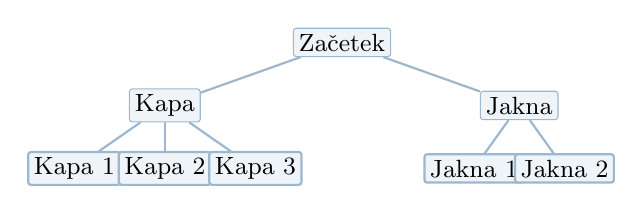
\begin{tikzpicture}[
    grow=down,
    level distance=8mm,
    level 1/.style={sibling distance=4.5cm},
    level 2/.style={sibling distance=1.15cm},
    every node/.style={
        draw=borderblue,
        rounded corners=1pt,
        fill=pale,
        inner sep=2pt,
        font=\small
    },
    edge from parent/.style={draw=borderblue, thick}
]
\node {Začetek}
    child {node {Kapa}
        child {node {Kapa 1}}
        child {node {Kapa 2}}
        child {node {Kapa 3}}
    }
    child {node {Jakna}
        child {node {Jakna 1}}
        child {node {Jakna 2}}
    };
\end{tikzpicture}
\end{center}
\textbf{Število listov:} \(3+2=5\) možnosti, kot napoveduje pravilo vsote.

\par\smallskip
\noindent\textcolor{borderblue}{\rule{\linewidth}{0.6pt}}
\smallskip

\textbf{\textcolor{navy}{Pravilo zmnožka -- »IN«.}}
Če se moramo odločiti za eno izmed $n_1$ izbir ene značilnosti, za eno izmed $n_2$ izbir druge značilnosti, . . . in eno izmed $n_k$ izbir k-te
značilnosti, pri čemer izbire nobene značilnosti niso odvisne od izbir drugih značilnosti, je skupno
število izbir:
\formula{n_1\cdot n_2\cdots n_k}
\zgled Na koliko načinov lahko oblečemo eno izmed 3 različnih kap in eno izmed 2 različnih
jaken?

\odgovor Od vsake skupine vzamemo eno izbiro (kapa IN jakna), zato možnosti zmnožimo. 
\racun \(3\cdot2=\mathbf{6}\) možnosti.

\par\smallskip
\noindent\textcolor{borderblue}{\rule{\linewidth}{0.6pt}}
\smallskip

\textbf{\textcolor{navy}{Kombinatorično drevo za pravilo zmnožka:}}
Drevo prikaže izbire po korakih: najprej izberemo kapo, nato jakno.
Vsaka pot od začetka do lista predstavlja eno možnost.
\begin{center}
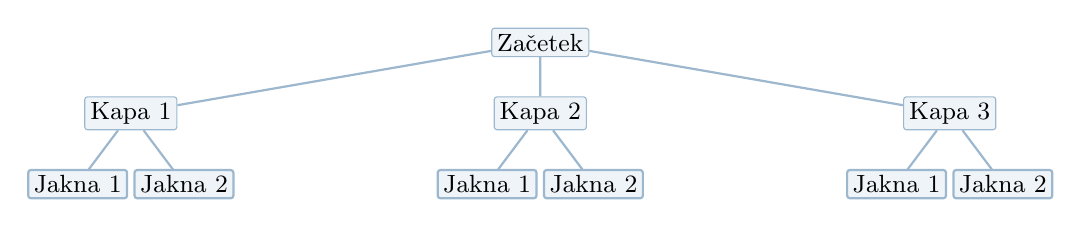
\begin{tikzpicture}[
    grow=down,
    level distance=9mm,
    level 1/.style={sibling distance=5.2cm},
    level 2/.style={sibling distance=1.35cm},
    every node/.style={
        draw=borderblue,
        rounded corners=1pt,
        fill=pale,
        inner sep=2pt,
        font=\small
    },
    edge from parent/.style={draw=borderblue, thick}
]
\node {Začetek}
    child {node {Kapa 1}
        child {node {Jakna 1}}
        child {node {Jakna 2}}
    }
    child {node {Kapa 2}
        child {node {Jakna 1}}
        child {node {Jakna 2}}
    }
    child {node {Kapa 3}
        child {node {Jakna 1}}
        child {node {Jakna 2}}
    };
\end{tikzpicture}
\end{center}
\textbf{Število listov:} \(2+2+2=6\), kar se ujema s pravilom
zmnožka \(3\cdot2=6\).
\end{topicbox}

\begin{topicbox}{2 \enspace Fakulteta}
Fakulteta števila \(n\) je produkt vseh pozitivnih celih števil do \(n\):
\formula{n!=n(n-1)\cdots2\cdot1,\qquad 0!=1}
\zgled Imamo 5 ljudi. Na koliko različnih načinov lahko zasedejo 5 stolov v vrsti?

\odgovor Za prvi stol je 5 možnosti, za naslednjega 4, nato 3, 2 in 1.
\racun \(5!=5\cdot4\cdot3\cdot2\cdot1=\mathbf{120}\) možnosti.
\end{topicbox}

\begin{topicbox}{3 \enspace Permutacije: razporejamo vse elemente}
Pri permutacijah uporabimo vse elemente ($n$), vrstni red pa je pomemben.
\begin{center}
\rowcolors{2}{pale}{white}
\begin{tabularx}{\linewidth}{>{\bfseries}p{3.3cm}p{4cm}X}
\toprule
Vrsta & Formula & Kdaj uporabimo?\\
\midrule
Brez ponavljanja & \(P_n=n!\) & Vsi elementi so različni.\\
S ponavljanjem &
\(\displaystyle P=\frac{n!}{r_1!r_2!\cdots r_k!}\) &
Nekateri elementi se ponavljajo; \(r_i\) je število ponovitev posameznega elementa.\\
\bottomrule
\end{tabularx}
\rowcolors{2}{}{}
\end{center}
\zgled Šest različnih oseb se postavi v vrsto.

\odgovor Razporedimo vseh 6 oseb. Na prvo mesto se lahko postavi katerakoli od 6 oseb. Na drugo mesto se lahko postavi le 5 oseb (ena oseba je že na prvem mestu). Za tretje mesto imamo 4 možnosti (oseb), za četrto 3, za peto 2 in za šesto mesto ostane le ena oseba, torej je le ena možnost. Za
zaporedna mesta je zato na voljo 6, 5, 4, 3, 2 in 1 možnosti.
\racun \(P_6=6!=6\cdot5\cdot4\cdot3\cdot2\cdot1=\mathbf{720}\).

\zgled Preštejmo različne razporeditve črk besede BANANA.

\odgovor Črka A se ponavlja, prav tako črka N. Če bi vse črke
razlikovali, bi dobili \(6!\) razporeditev (kar postavimo v števec), ker se pa črka A v besedi pojavi 3-krat, črka N pa 2-krat, delimo s $3!\cdot2!$ (imenovalec).
\racun \(\displaystyle\frac{6!}{3!\,2!}
=\frac{720}{6\cdot2}=\mathbf{60}\) različnih nizov.
\end{topicbox}

\begin{topicbox}{4 \enspace Variacije: izberemo in razporedimo del elementov}
Izberemo \(r\) elementov izmed \(n\); vrstni red je pomemben, izbranih
elementov pa ne uporabimo nujno vseh.
\begin{center}
\rowcolors{2}{pale}{white}
\begin{tabularx}{\linewidth}{>{\bfseries}p{3.3cm}p{4cm}X}
\toprule
Vrsta & Formula & Kdaj uporabimo?\\
\midrule
Brez ponavljanja &
\(\displaystyle V_n^r=\frac{n!}{(n-r)!}\) &
Izbrani elementi se ne smejo ponoviti.\\
S ponavljanjem & \(\overline{V}_n^r=n^r\) &
Element lahko izberemo večkrat.\\
\bottomrule
\end{tabularx}
\rowcolors{2}{}{}
\end{center}
\zgled Na koliko različnih načinov lahko med 10 dijaki podelimo zlato, srebrno in bronasto medaljo, vsako
drugemu dijaku?

\odgovor Medalje so različne, zato je vrstni red pomemben. Za zlato medaljo je
10 možnosti, nato 9 za srebrno in 8 za bronasto.
\racun \(V_{10}^3=10\cdot9\cdot8=\mathbf{720}\) možnosti za podelitev.

\zgled Koliko je možnosti za trimestno kodo iz 10 različnih števk; števke se lahko
ponavljajo?

\odgovor Koda ima tri mesta in na vsakem je 10 možnosti. Izbira na enem mestu
ne omeji izbire na drugih mestih.
\racun \(\overline{V}_{10}^3=10\cdot10\cdot10
=10^3=\mathbf{1000}\) kod.
\end{topicbox}

\begin{topicbox}{5 \enspace Kombinacije: izberemo skupino}
Izberemo \(r\) elementov izmed \(n\); vrstni red ni pomemben in elementi
se ne ponavljajo.
\formula{\binom{n}{r}=C_n^r=\frac{n!}{r!(n-r)!}}
\zgled Na koliko načinov lahko izmed 12 ljudi izberemo tričlansko komisijo?

\odgovor Izbira Ane, Borisa in Ceneta predstavlja isto komisijo kot izbira
Ceneta, Ane in Borisa. Vrstni red torej ni pomemben.
\racun
\[
    \binom{12}{3}
    =\frac{12\cdot11\cdot10}{3\cdot2\cdot1}
    =\mathbf{220}
\]
možnih komisij.

\zgled Na koliko načinov lahko izmed 8 fantov in 12 deklet izberemo četverico z natanko 2 dekletoma?

\odgovor Najprej izberemo 2 od 12 deklet, nato 2 od 8 fantov. Izbiri sta
neodvisni, zato števili možnosti zmnožimo.
\racun
\[
    \binom{12}{2}\binom{8}{2}
    =66\cdot28
    =\mathbf{1848}
\]
četveric.
\end{topicbox}

\begin{topicbox}{6 \enspace Kako izberemo pravi postopek?}
\begin{enumerate}
    \item Ugotovi, kaj šteješ: razporeditev, zaporedje ali skupino.
    \item Preveri, ali je vrstni red pomemben. Če ni, uporabi kombinacije.
    \item Ugotovi, ali razporejaš vse elemente (permutacije) ali le del
    (variacije oziroma kombinacije).
    \item Preveri, ali se elementi lahko ponavljajo.
    \item Pri več zaporednih stopnjah uporabi pravilo zmnožka; pri ločenih,
    medsebojno izključujočih se primerih pravilo vsote.
    \item Upoštevaj omejitve: primer razdeli na dovoljene možnosti ali od
    vseh možnosti odštej nedovoljene.
\end{enumerate}

\begin{center}
\rowcolors{2}{pale}{white}
\begin{tabularx}{0.9\linewidth}{>{\bfseries}p{3.5cm}XX}
\toprule
Kaj delamo? & Vrstni red pomemben & Vrstni red ni pomemben\\
\midrule
Razporejamo vse elemente & Permutacije & ---\\
Izbiramo le del elementov & Variacije & Kombinacije\\
\bottomrule
\end{tabularx}
\rowcolors{2}{}{}
\end{center}
\end{topicbox}

\begin{topicbox}{7 \enspace Binomski izrek in Pascalov trikotnik}
Binomski izrek razširi potenco dvočlenika. Koeficienti so binomski
koeficienti \(\binom{n}{k}\); dobimo jih tudi v \(n\)-ti vrstici
Pascalovega trikotnika:
\[
\begin{array}{ccccccccccc}
&&&&&1&&&&&\\
&&&&1&&1&&&&\\
&&&1&&2&&1&&&\\
&&1&&3&&3&&1&&\\
&1&&4&&6&&4&&1&\\
1&&5&&10&&10&&5&&1
\end{array}
\]
\formula{(a+b)^n=\sum_{k=0}^{n}\binom{n}{k}a^{n-k}b^k}
\((k+1)\)-ti člen binomskega razvoja (ne člen zaporedja) je
\formula{T_{k+1}=\binom{n}{k}a^{n-k}b^k,\qquad k=0,1,\ldots,n}

\zgled Določimo 4. člen razvoja \((2x-1)^6\).

\odgovor Ker iščemo 4. člen, velja \(k+1=4\), torej \(k=3\).
V formulo vstavimo \(n=6\), \(a=2x\) in \(b=-1\):
\[
    T_4
    =\binom{6}{3}(2x)^{6-3}(-1)^3
    =20\cdot8x^3\cdot(-1)
    =\mathbf{-160x^3}.
\]
Negativni predznak dobimo iz \((-1)^3=-1\).

\zgled Razvijmo \((x+2)^3\).

\odgovor Koeficienti v tretji vrstici Pascalovega trikotnika so \(1,3,3,1\).
Eksponent pri \(x\) pada od 3 do 0, pri 2 pa narašča od 0 do 3.
\racun
\[
    (x+2)^3
    =1x^3+3x^2\cdot2+3x\cdot2^2+1\cdot2^3
    =\mathbf{x^3+6x^2+12x+8}.
\]

\textbf{Postopek razvoja:} eksponent prvega člena zmanjšuj od \(n\) do 0,
eksponent drugega povečuj od 0 do \(n\), koeficiente vzemi iz
\(\binom{n}{k}\), nato poenostavi.
\end{topicbox}


\end{document}